\documentclass{article}

\usepackage{xetexko}
\usepackage{graphicx}

\title{정보보호 2주차: 카이사르\&비즈네르 암호}
\author{201704150 허강준}
\date{\today}

\begin{document}
    \maketitle
    
    \section{개요}
    고전암호는 인류 역사 중 주로 고대에서 중세 사이에 사용된 암호들을 일컫는다. 주로 전술, 전략이나 외교 문건과 같이 적대 세력이나 제 3자가 알지 말아야 할 정보들을 보호하기
    위하여 사용되었다. 잘 알려진 예 두가지로 카이사르 암호(시저 암호)와 비즈네르 암호가 있으며 본 보고서에서는 이 두 암호의 개략적인 작동 방식과 그 구현에 대해 다룬다.

    카이사르 암호는 율리어스 카이사르가 사용했다고 알려진 단순 대치 암호(Simple substitution cipher)의 일종이다. 모든 알파벳은 각각 다른 알파벳(혹은 키에 따라 같은 알파벳)과 1:1로
    대응된다. 키의 경우의 수는 0에서 25까지 총 26가지를 가질 수 있으며(혹은 -25까지 하여 51가지) 이 값만큼 떨어진 위치의 알파벳으로 대치한다. 
    
    \begin{figure}[!htbp]
        \centering
        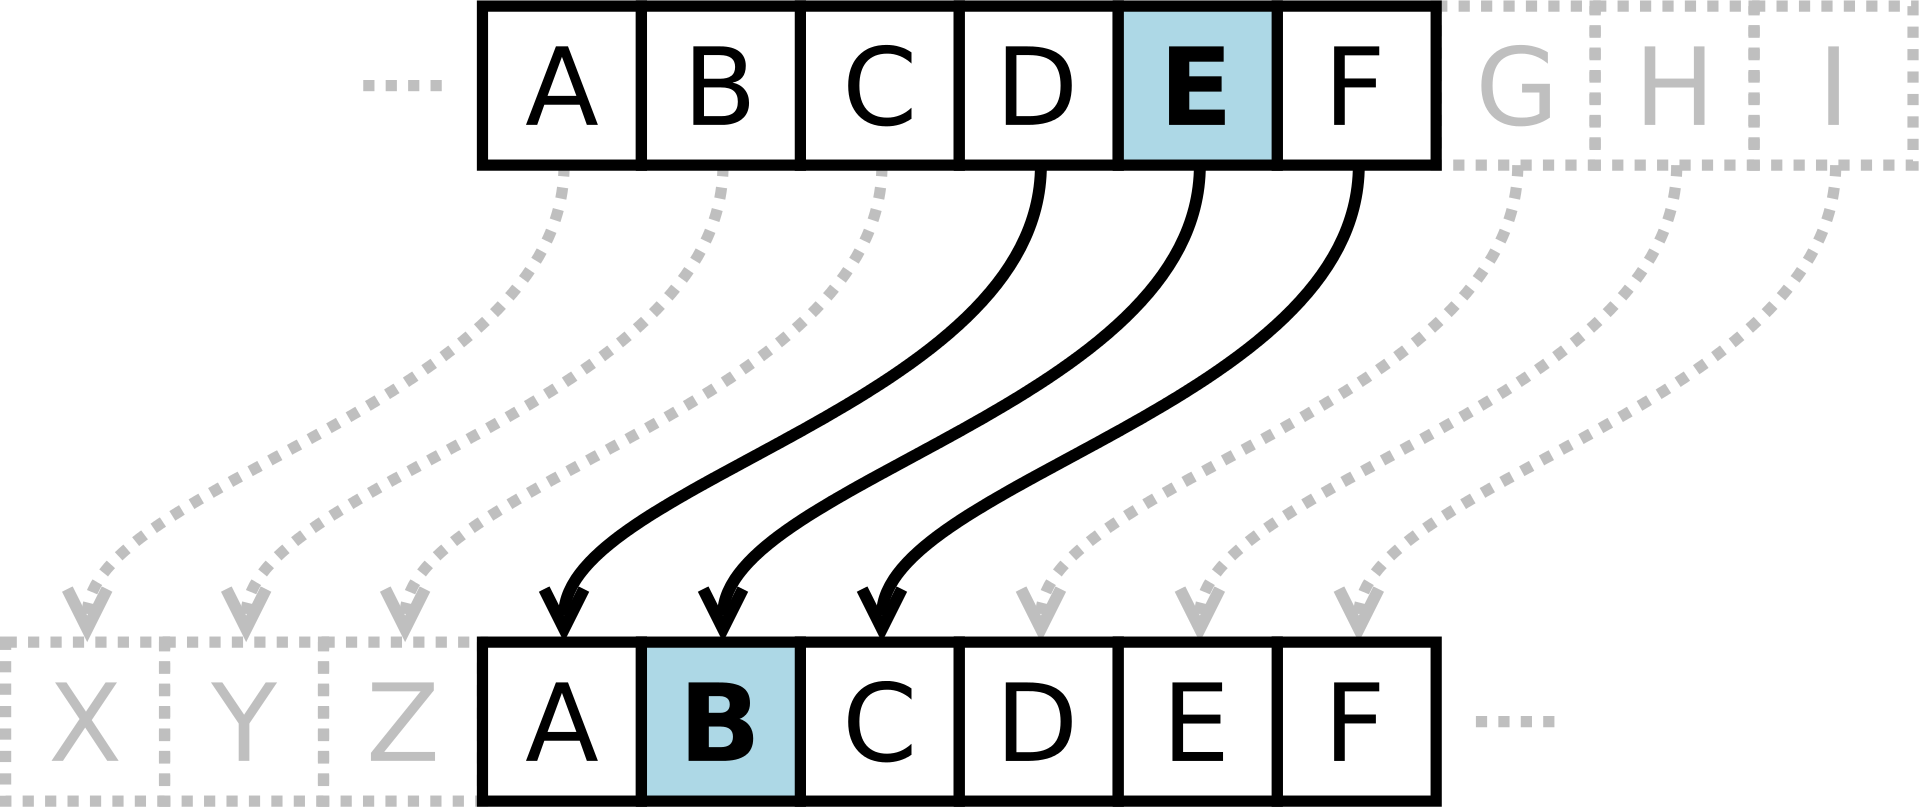
\includegraphics[width=0.6\textwidth]{image/caesar.png}
        \caption{카이사르 암호의 원리, 퍼블릭 도메인}
        \label{}
    \end{figure}

    또 다른 고전암호의 예시로 비즈네르 암호를 들 수 있다. 비즈네르 암호는 원래 Giovan Battista Bellaso가 개발하였으나
     Blaise de Vigenere의 이름을 따서 만들어진 암호로, 다중 대치 암호 (polyalphabetic substitution) 방식을 따른다. [2]
    키는 로마자로 표현될 수 있으며 이 키에 대응하면 알파벳에 대해 \textit{Vigenere Table} 혹은 \textit{tabula recta}라고 
    불리는 대치표를 사용한다. 만일 키가 전체 평문보다 짧은 경우 키의 처음 문자부터 다시 진행하며 이러한 과정을 통해 같은 평문에
    대하여 다른 문자가 대응되어 추측을 어렵게 할 수 있다.

    \section{구현}
    Python을 이용하여 구현하였다. 실제 구현체는 예시와는 다르게 A에서 Z 까지 뿐만이 아닌 소문자, 숫자에 대한 암/복호화도 지원해야
    했다. 두 알고리즘 보드 사전에 \texttt{lower\_alphabet\_list}, \texttt{upper\_alphabet\_list}, 그리고 \texttt{number\_list}가
    제공되어 상황에 맞게 해당 리스트들을 교체하여 사용하는 방식으로 구현하였다. 

    \subsection{카이사르 암호}
    카이사르 암호는 단순 대치 암호이므로 단순히 해당 위치의 ASCII 상대 위치(-'A', -'a', - '0')를 구한 뒤 \texttt{key} 만큼 더해주었다.
    문자 대역을 넘어가는 경우 처음부터 다시 진행하므로 해당 문자 대역 내 존자하는 문자의 갯수로 modulo 연산을 수행하였다.

    \subsection{비즈네르 암호}
    비즈네르 암호의 경우 \texttt{ENC}, \texttt{DEC} 라는 두가지 모드를 파라메터로서 받는다. 암호화의 역이 복호화이므로, \texttt{enc\_mode}
    라는 변수에 해당 파라메터의 값에 따라 1 혹은 -1을 대입하여 활용하였다. 이 변수는 \texttt{key}에 곱해지는 값으로 복호화 시
    키를 음수로 바꾸어 복호화가 가능하도록 하였다.

    카이사르 암호와는 다르게 비즈네르 암호는 키의 길이를 다르게 할 수 있고, 평문이 키보다 긴 경우가 많아 암/복호화 처리시에 키 중의 문자들 중에서
    어떤 문자를 선택할 것인가에 대한 고려가 필요하였다. 이것은 현재 평문 인덱스를 키 길이로 modulo 연산을 통해 해결할 수 있었다.

    \section{테스트}
    테스트는 pytest를 이용하여 진행되었다. 사전에 작성되어 제공된 실습용 테스트 케이스를 이용하여 테스트하였으며, 이후
    레포지토리에 push 하여 최종 테스트를 통과하였음을 확인하였다.

    \section{결론}
    카이사르 암호 및 비즈네르 암호는 단순 혹은 다중 대치 암호의 대표적인 예시로서, 암호를 만드는 방법에 대해 간략하게 알아 볼 수
    있는 대표적인 예시라고 할 수 있다. 현대에는 이들 암호의 유명세에 걸맞게 그 취약점 또한 잘 알려져 있어 중요한 일에 사용하기에는
    무리가 따를 것이다.


    \section*{참고문헌}
        \begin{itemize}
            \item [1] Bellaso, Giovan Battista (1553). \textit{La Cifra del Sig.}
            \item [2] Bruen, Aiden A. \& Forcinito, Mario A. (2011). \textit{Cryptography, Information Theory, and Error-Correction: A Handbook for the 21st Century. John Wiley \& Sons.} p. 21. ISBN 978-1-118-03138-4. 
        \end{itemize}
\end{document}